\begin{frame}
\frametitle{Продвинутые алгоритмы аллокации памяти}
\framesubtitle{Аллокация в несколько этапов}

Современные аллокаторы памяти выделяют две стадии:

\begin{itemize}
  \item<2-> аллокация больших блоков (Buddy Allocator и Ко.):
    \begin{itemize}
      \item аллокации происходят нечасто, большие объекты живут долго
      \item чем больше блок тем меньше накладные расходы на служебные структуры аллокатора - можем хранить больше информации
    \end{itemize}
  \item<3-> аллокация маленьких блоков фиксированного размера (SLAB и Ко.):
    \begin{itemize}
      \item блоки фиксированного размера проще аллоцировать
      \item блоки фиксированного размера требуют меньше служебной информации
      \item блоки имеют одинаковый размер не случайно - часто это объекты одного типа и это можно использовать
    \end{itemize}
\end{itemize}

\end{frame}

\begin{frame}
\frametitle{Buddy Allocator}
\framesubtitle{Вводные положения}

\begin{itemize}
  \item вся аллоцируемая память разбита на большие блоки фиксированного размера (будем называть их PAGE)
  \item каждому PAGE поставлен в соответствие дескриптор (мы легко можем получить дескриптор по номеру PAGE и наоборот, считайте, что у нас есть массив таких дескрипторов), хранящий служебную информацию (свободен/занят, порядок свободного блока)
  \item память аллоцируется и освобождается блоками по $2^i\times PAGE$, $i$ будем называть порядком блока
  \item порядок блока хранит пользователь и передает его в как функцию аллокации, так и в функцию освобождения
\end{itemize}
\end{frame}

\begin{frame}
\frametitle{Buddy Allocator}
\framesubtitle{Buddies}

Ключевой концепцией для Buddy Allocator-а является понятие Buddy:
\begin{itemize}
  \item Buddy Allocator хранит блоки в отдельных списках для каждого порядка (т. е. для каждого возможного порядка блока есть свой список), элементом списка является дескриптор первого PAGE в этом блоке;
  \item смежные (в памяти, а не в списке) блоки одного порядка называются Buddies (plural for buddy);
  \item два смежных блока (Buddies) в объединении дают один блок большего порядка, и наоборот из одного блока можно получить два Buddies меньшего порядка.
\end{itemize}

\end{frame}

\begin{frame}
\frametitle{Buddy Allocator}
\framesubtitle{Buddies}

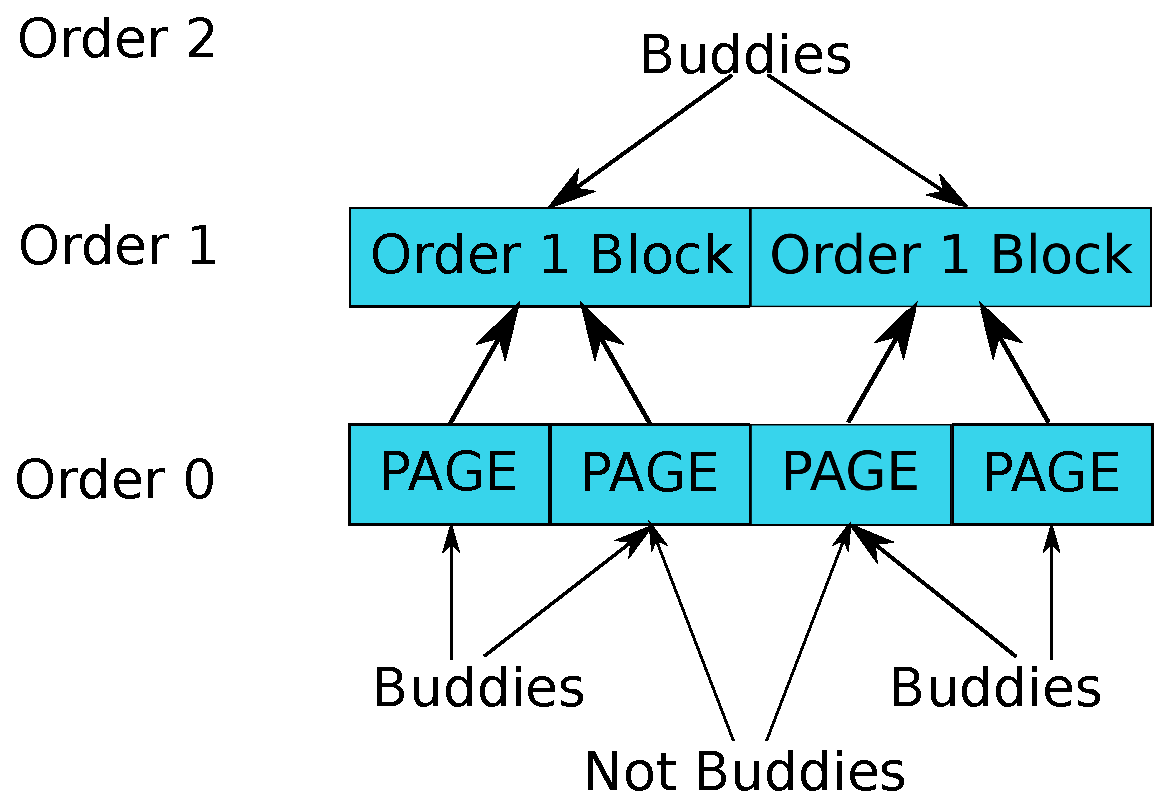
\includegraphics[width=.9\linewidth]{buddy-buddies}

\end{frame}

\begin{frame}
\frametitle{Buddy Allocator}
\framesubtitle{Аллокация}

Аллокация блока порядка $i$ происходит из списка соответствующего блокам порядка $i$:

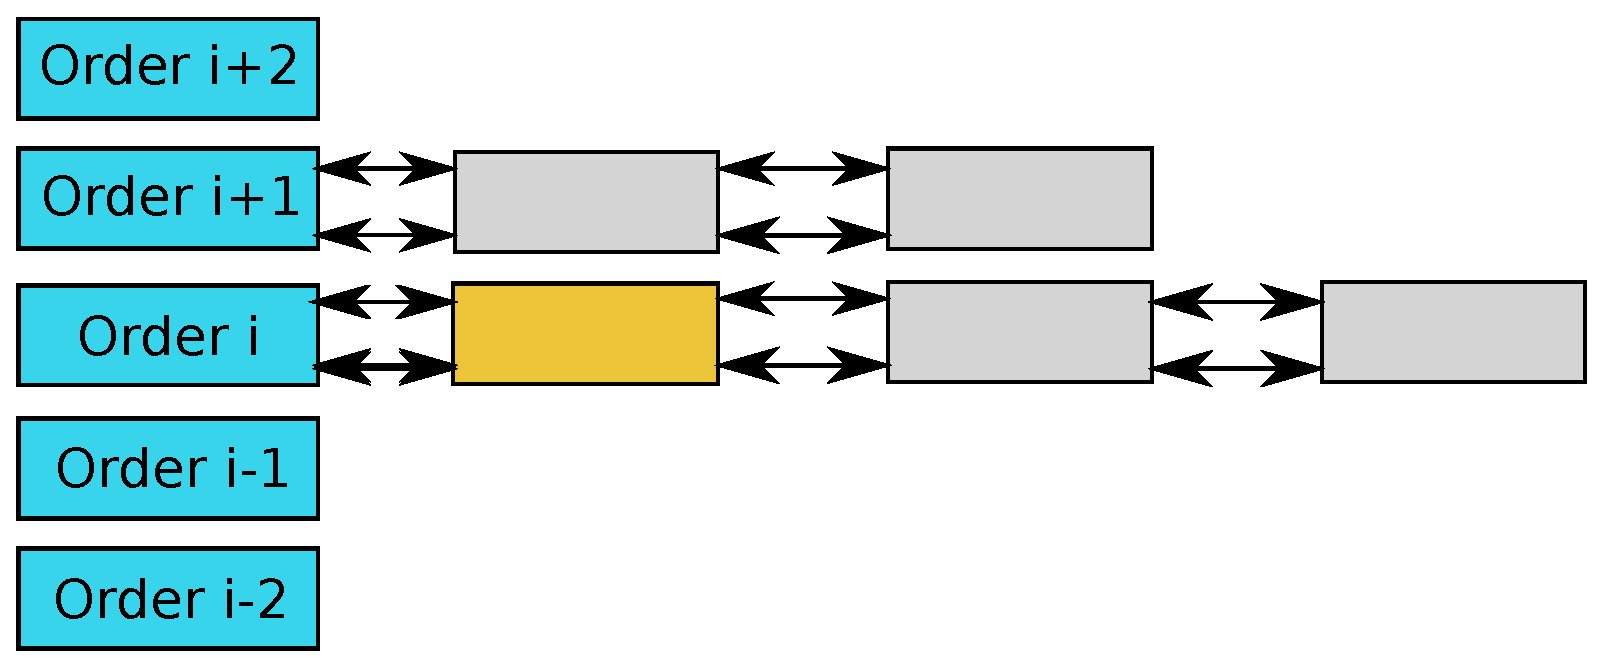
\includegraphics[width=.9\linewidth]{buddy-alloc0}

\end{frame}

\begin{frame}
\frametitle{Buddy Allocator}
\framesubtitle{Аллокация}

Если список пуст, ищем не пустой список большего порядка и аллоцируем из него, например, аллоцируем блок порядка $i-2$:

\includegraphics[width=.8\linewidth]{buddy-alloc1}

\end{frame}

\begin{frame}
\frametitle{Buddy Allocator}
\framesubtitle{Аллокация}

Блок порядка $i$ слишком большой, поэтому делим его на две части порядка $i-1$ и одну из частей возвращаем аллокатору:

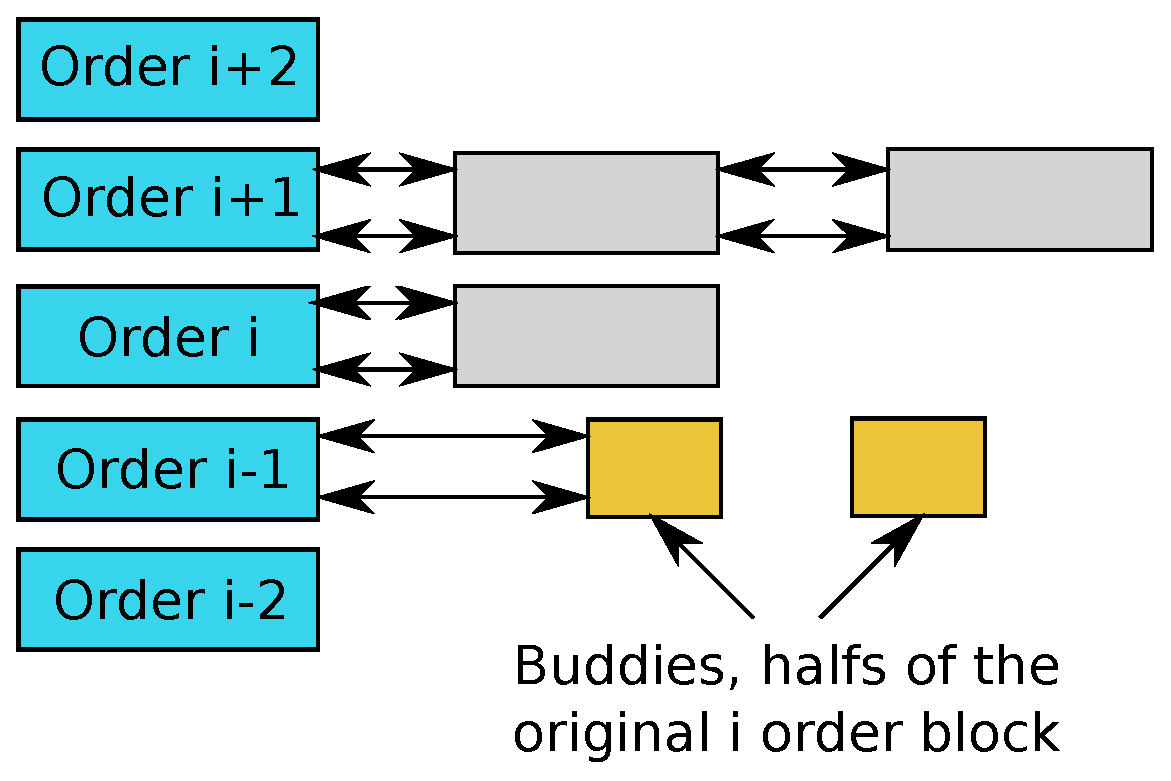
\includegraphics[width=.8\linewidth]{buddy-alloc2}

\end{frame}

\begin{frame}
\frametitle{Buddy Allocator}
\framesubtitle{Аллокация}

Продолжаем пока не дойдем до нужного порядка:

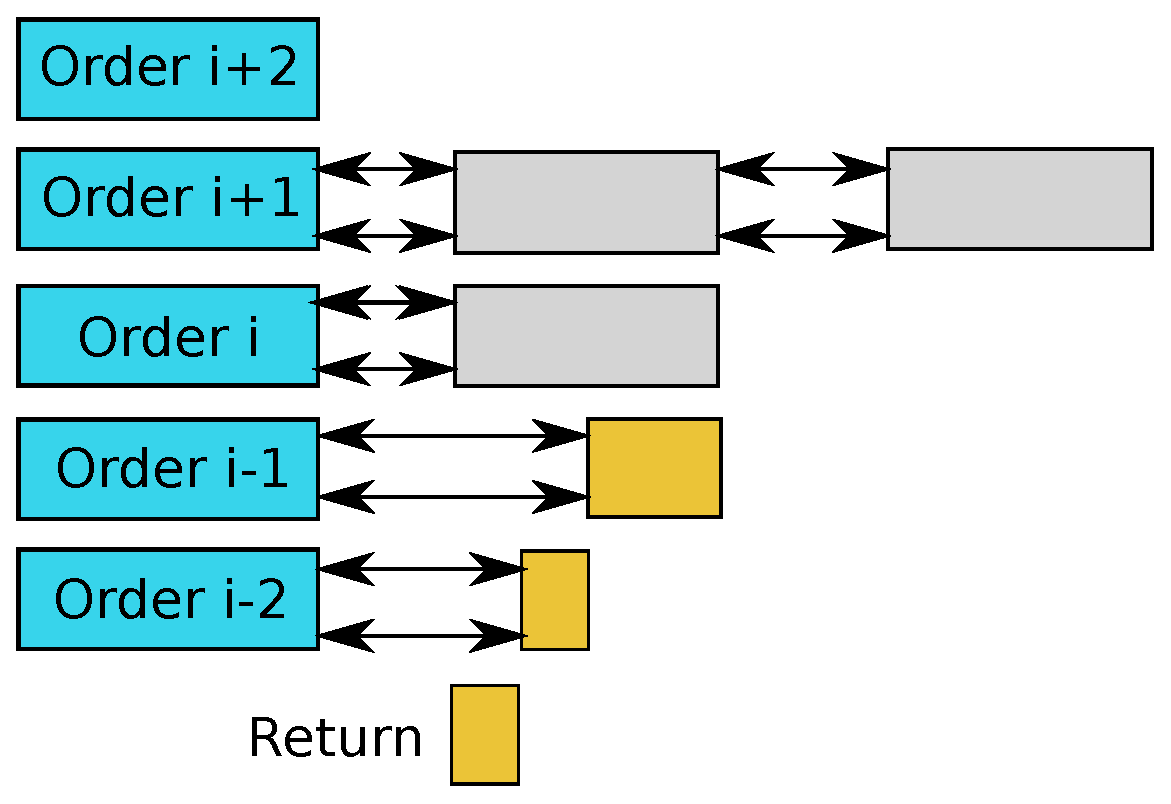
\includegraphics[width=.8\linewidth]{buddy-alloc3}

\end{frame}

\begin{frame}
\frametitle{Buddy Allocator}
\framesubtitle{Аллокация}

Каждый свободный блок, как отмечалось выше представляется дескриптором первого PAGE, дескриптор должен хранить:

\begin{itemize}
  \item признак занятости и свободности блока;
  \item порядок блока, "головой" которого является данный PAGE.
\end{itemize}

Эта информация не нужна для аллокации, но понадобится для освобождения, поэтому
при разделении блока необходимо обновить дескрипторы обоих половин.

\end{frame}

\begin{frame}
\frametitle{Buddy Allocator}
\framesubtitle{Освобождение}

При освобождении необходимо объединять смежные блоки (Buddies), чтобы избежать фрагментации. Найти "голову" смежного блока легко:

\[
	Buddy_{No} = Head_{No} \char`\^ (1 << i)
\]

где
\begin{itemize}
  \item $Buddy_{No}$ - номер PAGE, являющегося "головой" смежного блока;
  \item $Head_{No}$ - номер PAGE, являющегося "головой" блока, с которым мы работаем;
  \item $i$ - порядок блока;
\end{itemize}

\end{frame}

\begin{frame}
\frametitle{Buddy Allocator}
\framesubtitle{Освобождение}

Освобождаемый блок можно объединить со смежным (Buddy), только если смежный блок свободен. Смежный блок свободен если:

\begin{itemize}
  \item в дескрипторе "головы" блока установлен признак свободности;
  \item порядок сохраненный в дескрипторе "головы" блока совпадает с порядком освобождаемого блока.
\end{itemize}
\end{frame}

\begin{frame}
\frametitle{Buddy Allocator}
\framesubtitle{Освбождение}

Прядок блоков важен при объединении:
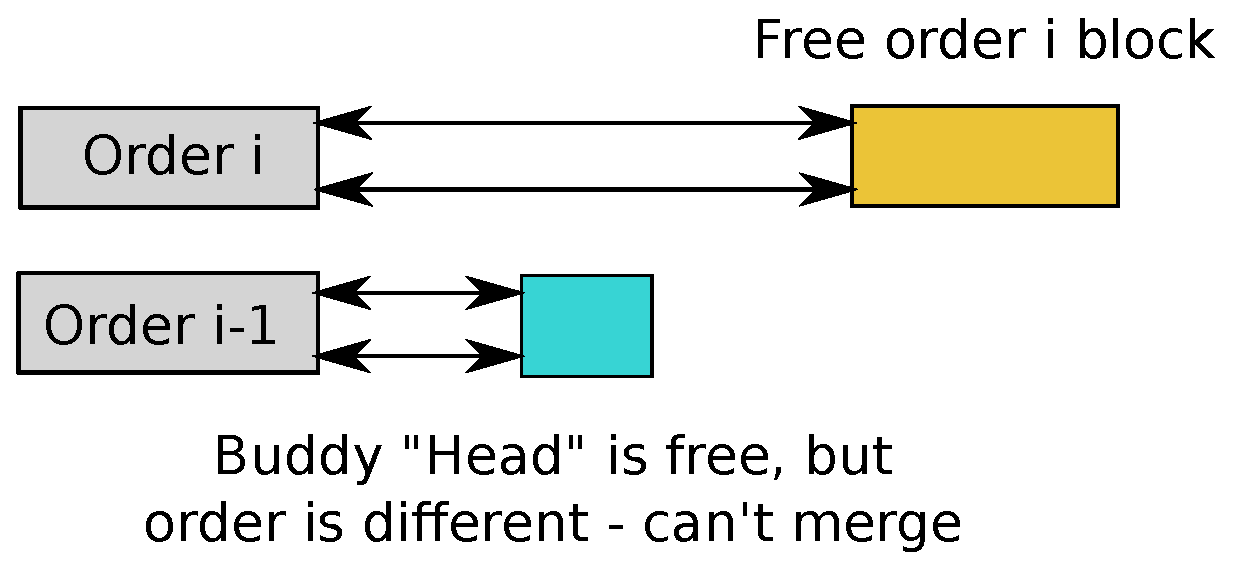
\includegraphics[width=.9\linewidth]{buddy-free0}
\end{frame}

\begin{frame}
\frametitle{Buddy Allocator}
\framesubtitle{Освобождение}

Возможно придется сделать несколько объединений:
\only<1>{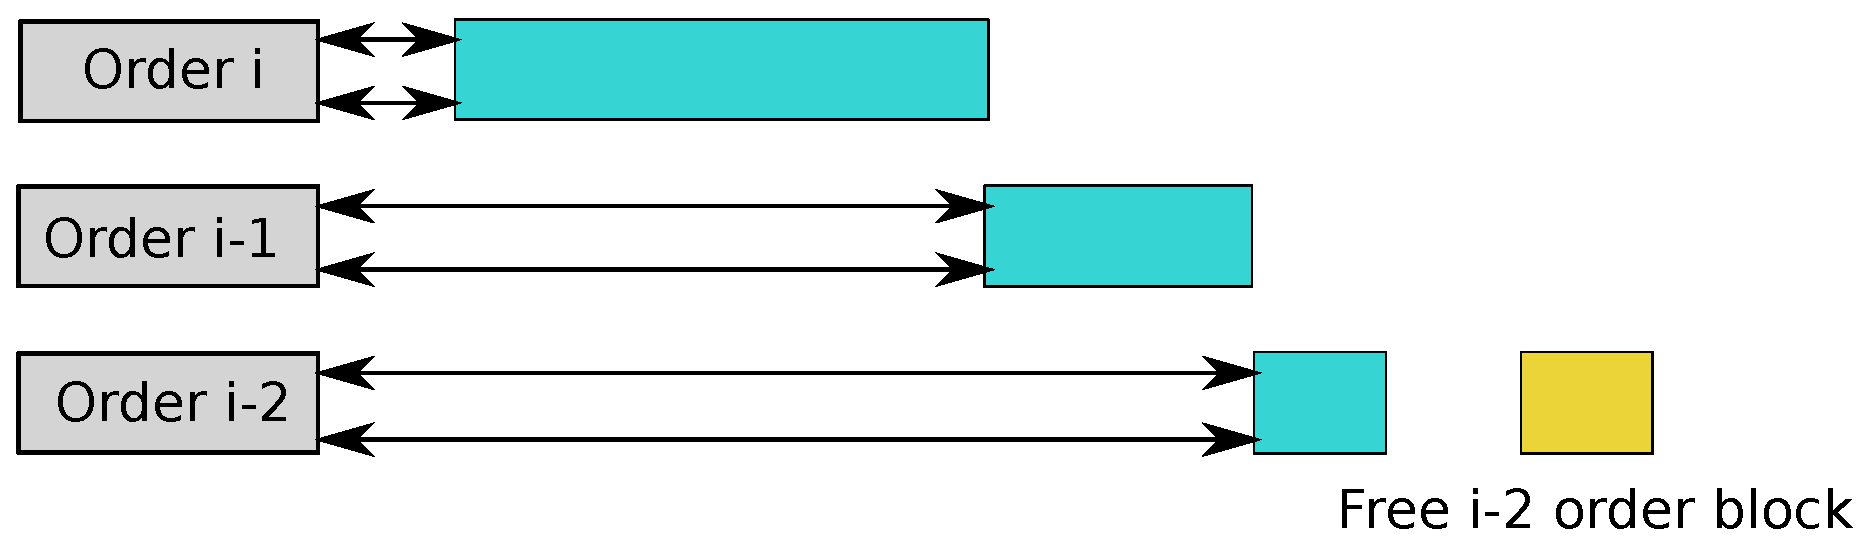
\includegraphics[width=.9\linewidth]{buddy-free1}}
\only<2>{\includegraphics[width=.9\linewidth]{buddy-free2}}
\only<3>{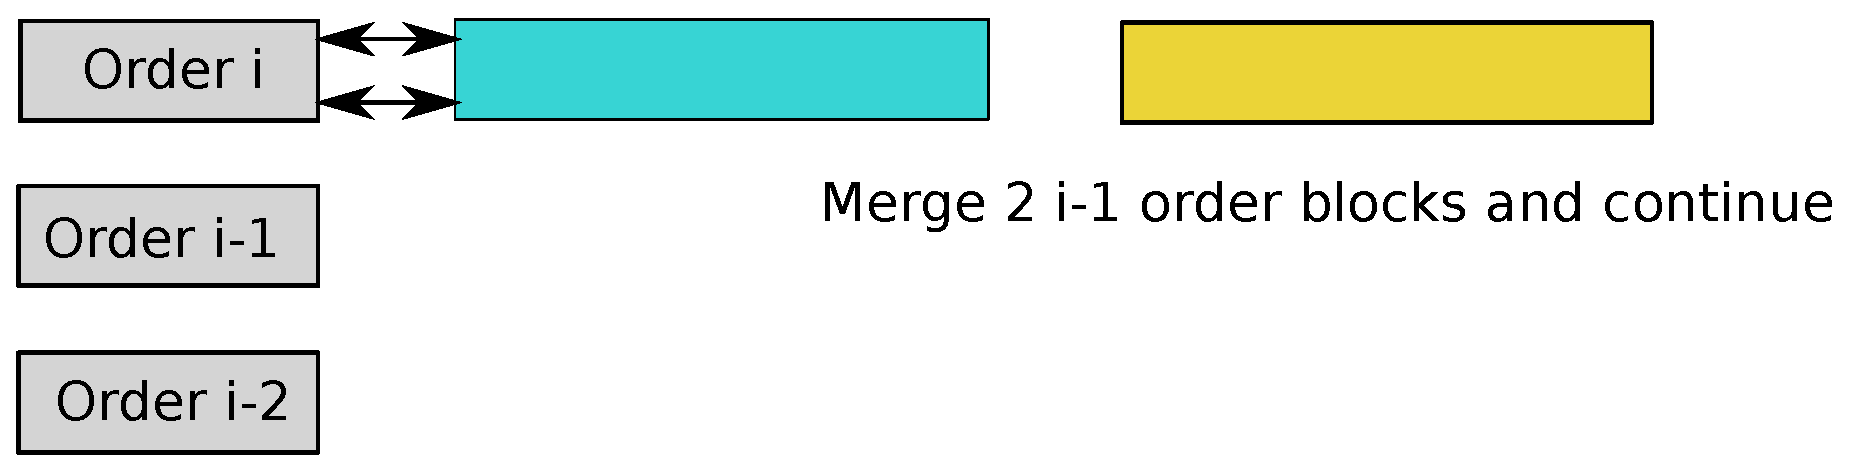
\includegraphics[width=.9\linewidth]{buddy-free3}}

\end{frame}

\begin{frame}
\frametitle{Buddy Allocator}
\framesubtitle{Освобождение}

Продолжаем пока можем объединять смежные блоки или не дойдем до последнего уровня:
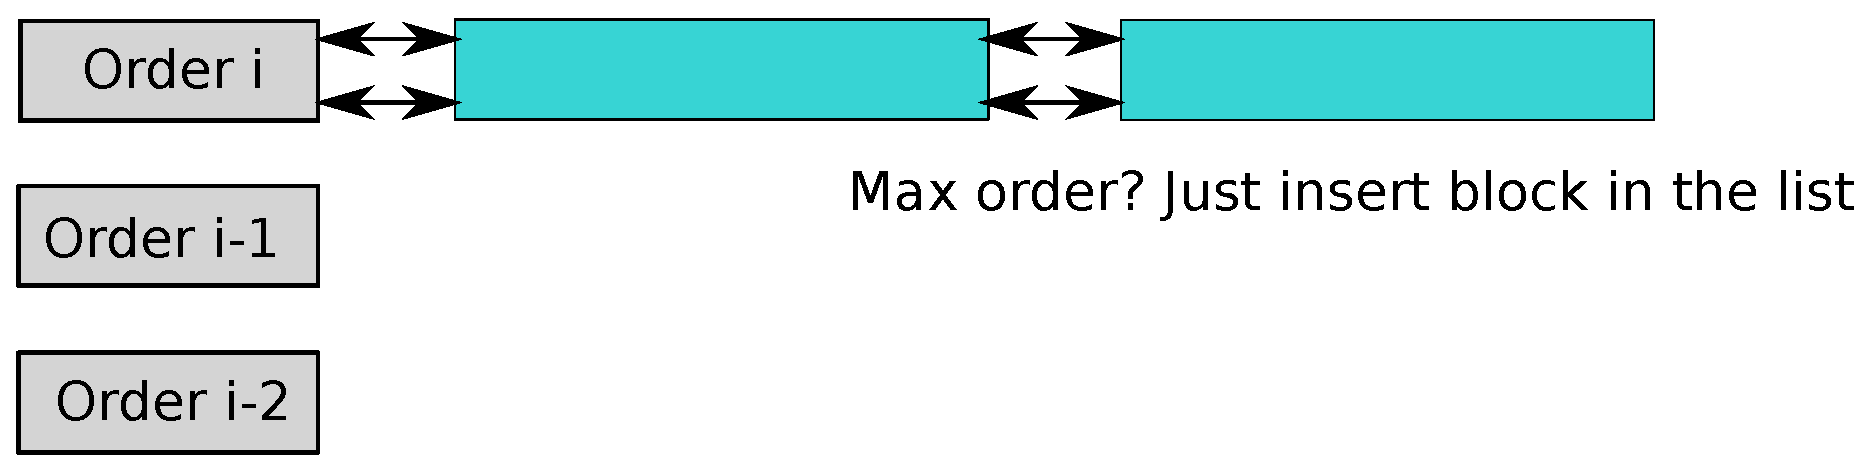
\includegraphics[width=.9\linewidth]{buddy-free4}
\end{frame}

\begin{frame}
\frametitle{Buddy Allocator}
\framesubtitle{Аллокация блоков произвольного размера}

Аллокация блоков только по степеням 2 может быть затратной - в неудачных случаях мы аллоцируем почти в 2 раза больше чем нужно. Есть как минимум 2 решения этой проблемы:

\begin{itemize}
  \item пожертвовать интерфейсом - разложить количество блоков на сумму степеней 2 и аллоцировать каждый блок размера $2^i$ отдельно и возвращать массив блоков;
  \item поправить алгоритм для аллокация блоков произвольного размера;
\end{itemize}
\end{frame}

\begin{frame}
\frametitle{Buddy Allocator}
\framesubtitle{Аллокация блоков произвольного размера}

Buddy Allocator легко изменить для аллокации блоков произвольного размера пожертвовав (совсем немного) памятью:
\begin{itemize}
  \item вместо порядка блока в дескрипторе PAGE храним размер (очевидно);
  \item храним признак занятости/свободности и размер как в дескрипторе первого PAGE блока, так и в дескрипторе последнего (Border Tags);
  \item каждый список хранит блоки размеров $\left[2^i;2^{i+1}\right)$, кроме последнего - для него нет верхней границы.
\end{itemize}
\end{frame}
